\begin{frame}{Higgs production modes}
    \begin{figure}
        \centering
        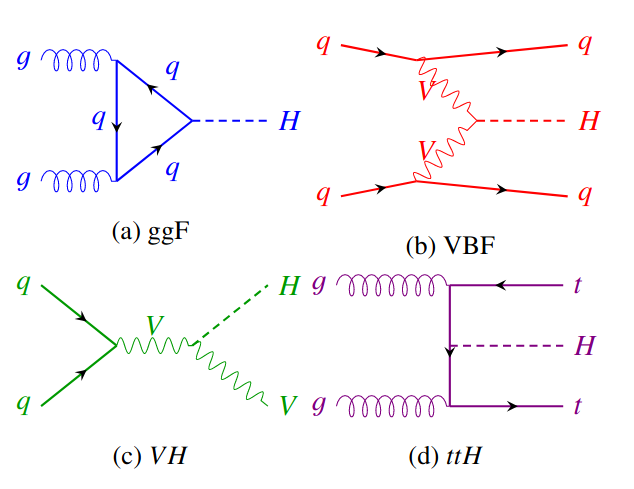
\includegraphics[width=0.6\textwidth]{BackUp/Part1/Img/Higgs_prod_modes.png}
        
    \end{figure}
\end{frame}

\begin{frame}{Higgs cross-section}

\begin{figure}
    \centering
    \subfloat{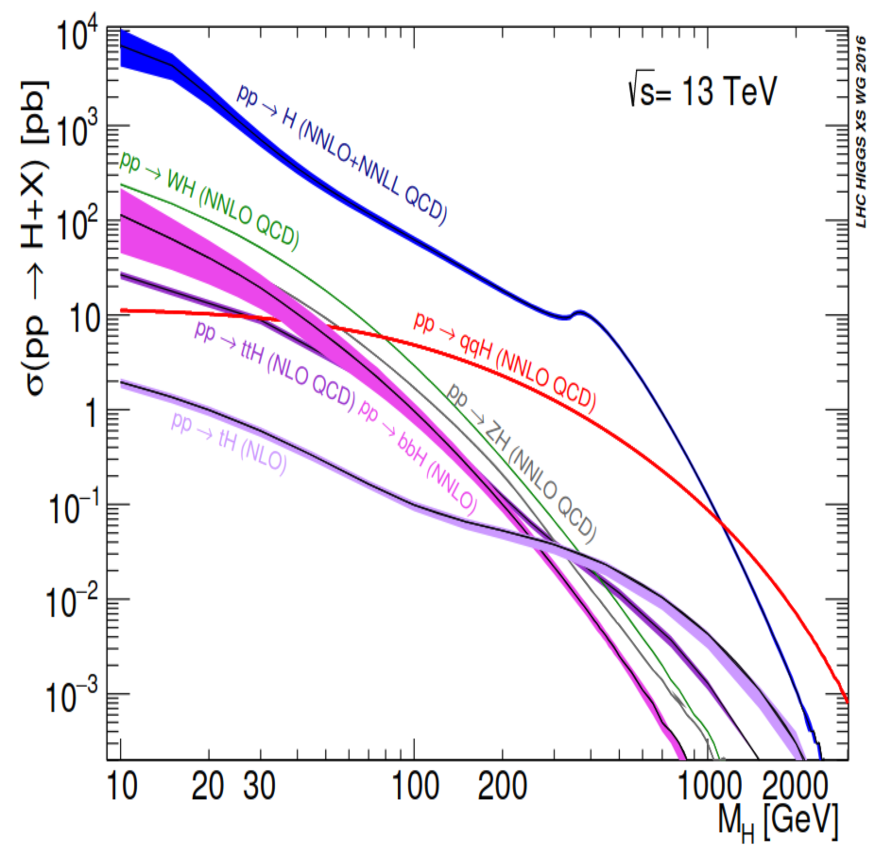
\includegraphics[width=0.5\textwidth]{BackUp/Part1/Img/Higgs_Xsec_mass.png}} 
    \subfloat{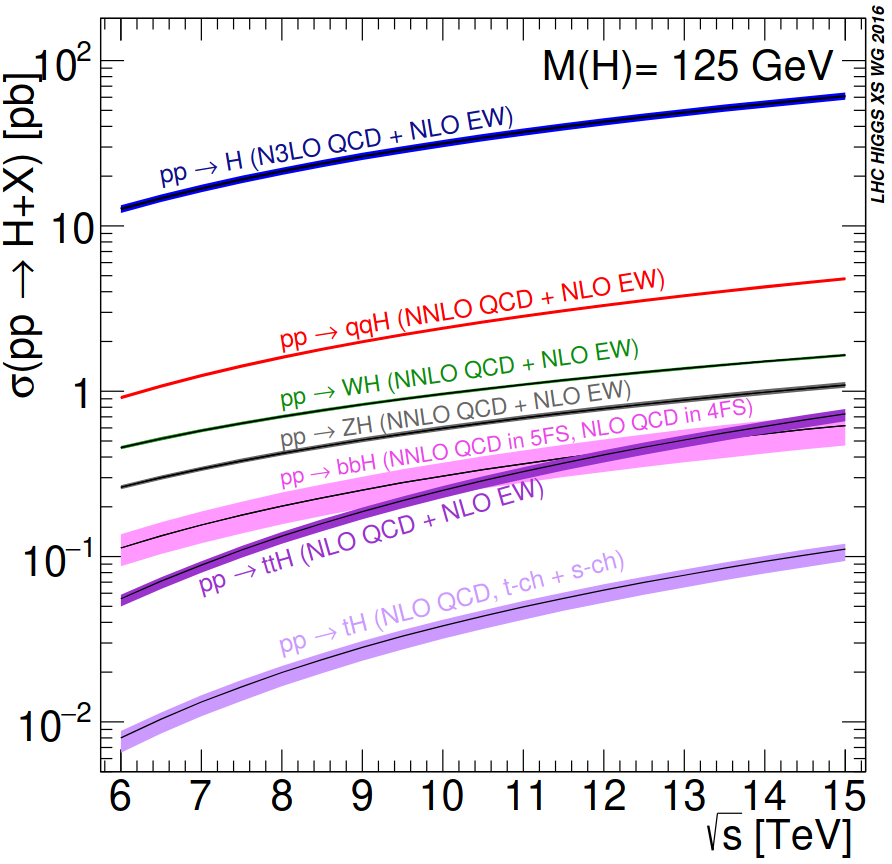
\includegraphics[width=0.5\textwidth]{BackUp/Part1/Img/Higgs_Xsec_s.png}}
\end{figure}
    
\end{frame}

\begin{frame}{Higgs decay modes}
    
\begin{figure}
    \centering
    \subfloat{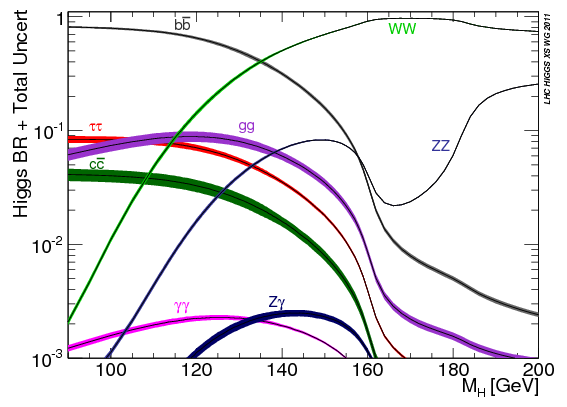
\includegraphics[width=0.5\textwidth]{BackUp/Part1/Img/Higgs_Br.png}} \\
    \subfloat{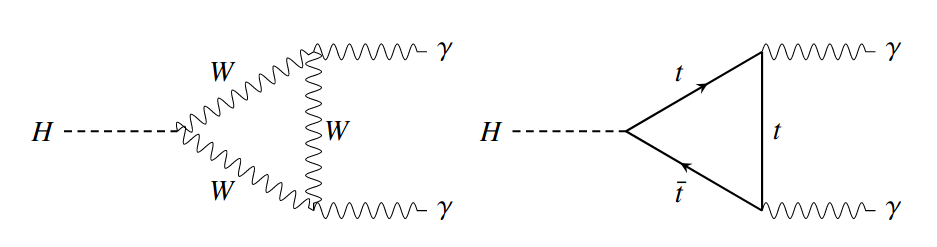
\includegraphics[width=0.5\textwidth]{BackUp/Part1/Img/H_to_gammagamma.png}}
\end{figure}
\end{frame}

\begin{frame}{Higgs self-coupling}
\begin{figure}
    \centering
    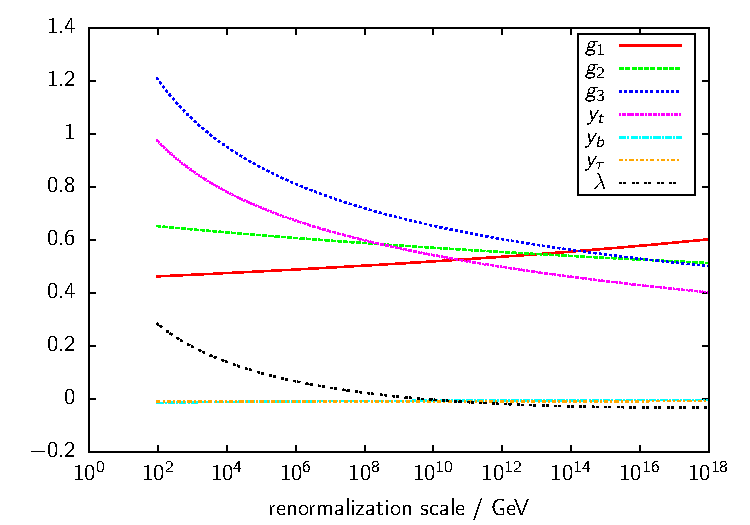
\includegraphics[width=.7\textwidth]{BackUp/Part1/Img/SM_rgflow.pdf}
\end{figure}    
    
\end{frame}

\begin{frame}{Di-Higgs pheomonology}
\begin{figure}
    \centering
    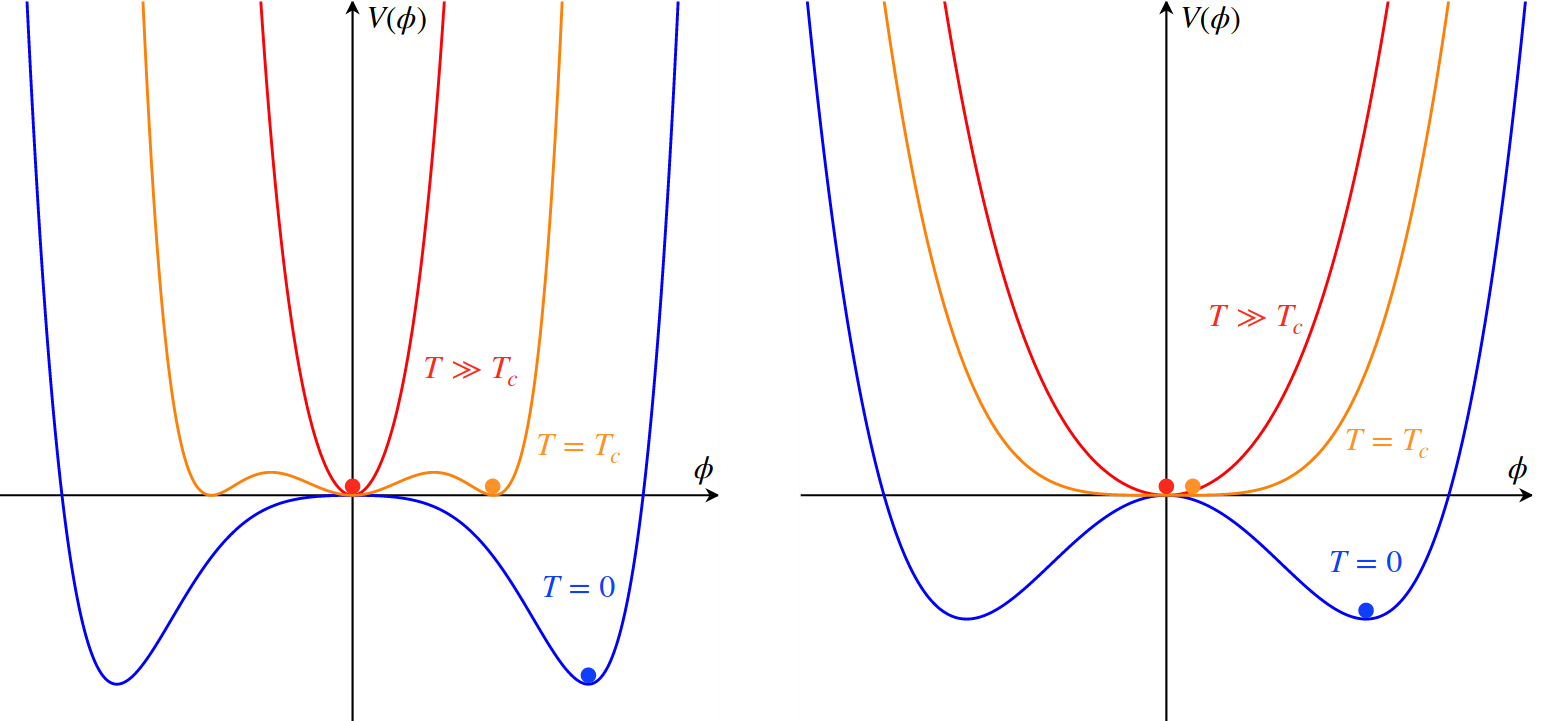
\includegraphics[width=1.\textwidth]{BackUp/Part1/Img/Higgs_shape_T.png}
\end{figure}
\end{frame}

\begin{frame}{Di-Higgs cross-section}

\begin{equation*}
    A(\lambda_t, \lambda_{HHH}) \equiv \lambda_t^2\cdot\square + \lambda_t\cdot\lambda_{HHH}\bigtriangleup
\end{equation*}

\begin{equation*}
  \sigma \approx k_{t}^{4}\left[|\square|^{2}+\frac{k_{\lambda}}{k_{t}}(\square\bigtriangleup+\bigtriangleup \square)+\left(\frac{k_{\lambda}}{k_{t}}\right)^{2}|\bigtriangleup|^{2}\right]
  \label{eq:chap1:HH:XSEC:Param}
\end{equation*}

\begin{itemize}
    \item minimum cross-section at $\kappa_{\lambda} = 2.4 \kappa_{t}$
    \item minimum $m_{HH}$ at $m_{HH} = 2 m_{t}$ for $\kappa_{\lambda} = 2$
    \item $\sigma_{\text{ggF HH}}^{\text{NNLO}} = 31.05_{-5.0\%}^{+2.2\%}$ fb
    \item $\sigma_{\text{VBF HH}}^{\text{NNLO}} = 1.723_{-0.04\%}^{+0.03\%} \ \text{fb}$
\end{itemize}
\begin{table}[]
    \centering
    \begin{tabular}{cccc}
    \hline\hline
     per $t$ & 1 H per 1s & 3 HH per 1h & 1 HH($b\bar{b}\gamma\gamma$) per 5d  \\
     per $pp$ & 2.5 10$^{-9}$ H & 2 10$^{-11}$ HH &  6.25 10$^{-16}$ 2H \\
    \hline\hline    
    \end{tabular}
\end{table}

\end{frame}

\begin{frame}{Di-Higgs production modes}
    \begin{figure}
        \centering
        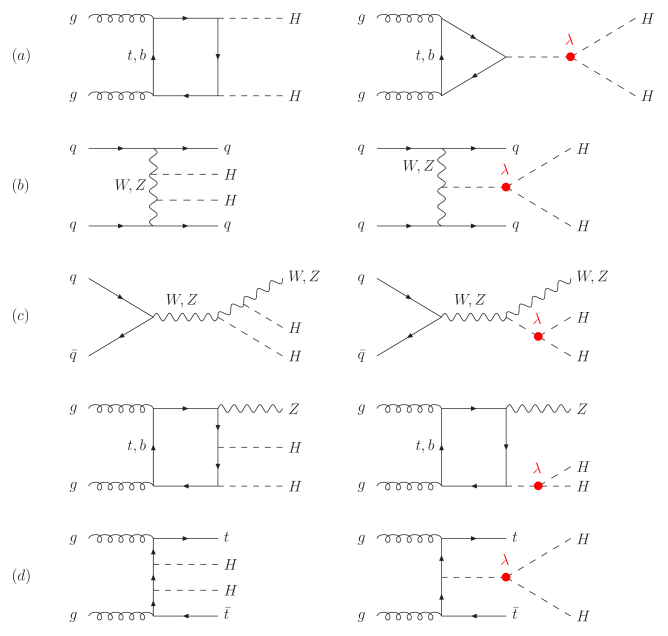
\includegraphics[width=0.6\textwidth]{BackUp/Part1/Img/HH_feyns.png}
        
    \end{figure}
\end{frame}
\begin{frame}{Di-Higgs cross-section as function of $\sqrt{s}$}
\begin{figure}
    \centering
    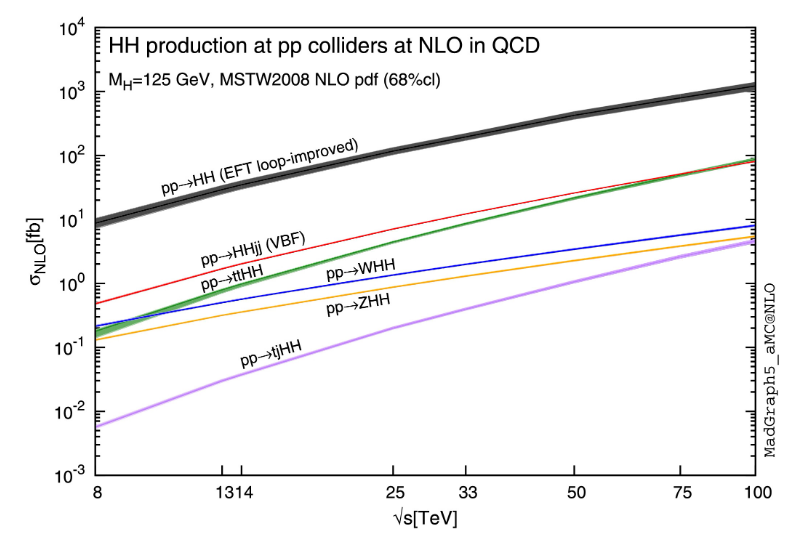
\includegraphics[width=0.8\textwidth]{BackUp/Part1/Img/HH_XSec_as_S.png}
\end{figure}
\end{frame}